\documentclass[12pt,a4paper]{article}

\usepackage{iftex}
\ifPDFTeX
    \usepackage[T2A]{fontenc}
    \usepackage[utf8]{inputenc}
    \usepackage[russian]{babel}
    \usepackage{cmap}
\else
    \usepackage{fontspec}
    \setmainfont{Times New Roman}
    \setmonofont{Courier New}
    \usepackage{polyglossia}
    \setdefaultlanguage{russian}
    \newfontfamily\cyrillicfont{Times New Roman}[Script=Cyrillic]
    \newfontfamily\cyrillicfonttt{Courier New}
\fi

\usepackage[left=25mm,right=20mm,top=20mm,bottom=20mm]{geometry}
\usepackage{amsmath,amssymb}
\usepackage{graphicx}
\usepackage{float}
\usepackage{array}
\usepackage{booktabs}
\usepackage{indentfirst}
\usepackage{enumitem}
\usepackage{fvextra}
\usepackage[hidelinks]{hyperref}

\graphicspath{{lab2/}{lab3/}}
\hypersetup{
    pdftitle={Отчёт по предмету «Численные методы»},
    pdfauthor={Ситников И. А.}
}
\setlength{\parindent}{1.25cm}
\setlength{\parskip}{0pt}
\setlength{\emergencystretch}{2em}
\renewcommand{\arraystretch}{1.15}
\renewcommand{\contentsname}{Содержание}
\pagestyle{plain}

\newcommand{\eps}{\varepsilon}
\newcommand{\codeinput}[1]{%
    \VerbatimInput[
        fontsize=\footnotesize,
        breaklines=true,
        breakanywhere=true,
        tabsize=4
    ]{#1}%
}
\newcommand{\programwithoutput}[2]{%
    \codeinput{#1}
    \vspace{5mm}
    \noindent\textbf{Вывод программы:}
    \vspace{2mm}
    \codeinput{#2}
}

\begin{document}

\hypersetup{pageanchor=false}
\begin{titlepage}
    \centering
    {\large МОСКОВСКИЙ АВИАЦИОННЫЙ ИНСТИТУТ\par}
    \vspace{3mm}
    {\large (НАЦИОНАЛЬНЫЙ ИССЛЕДОВАТЕЛЬСКИЙ УНИВЕРСИТЕТ)\par}
    \vspace{8mm}
    {\normalsize Институт №8 «Компьютерные науки и прикладная математика»\par}
    {\normalsize Кафедра №806 «Вычислительная математика и программирование»\par}

    \vfill
    {\Large\bfseries Отчёт\par}
    \vspace{2mm}
    {\large\bfseries по предмету «Численные методы»\par}

    \vfill
    \begin{flushright}
        \begin{tabular}{@{}ll@{}}
            Выполнил: & Ситников И.\,А.\\
            Группа: & М8О-307Б-23\\
            Преподаватель: & Киндинова В.\,В.\\
            Вариант: & 24
        \end{tabular}
    \end{flushright}

    \vfill
    {\large Москва 2026\par}
\end{titlepage}
\hypersetup{pageanchor=true}
\setcounter{page}{2}

\tableofcontents
\clearpage

\section{Решение СЛАУ}

\subsection{Задание 1.1}

\subsubsection{Формулировка задания}
Реализовать алгоритм $LU$-разложения матриц с выбором главного элемента.
Используя разработанную программу, решить систему линейных алгебраических
уравнений, вычислить определитель матрицы системы и обратную матрицу.

\subsubsection{Вариант № 24}
Решить систему $Ax=b$, где
\[
A=\begin{pmatrix}
 7&-5& 6& 7\\
 8&-1&-9& 1\\
-3& 8& 8& 8\\
 2&-3& 6&-4
\end{pmatrix},
\qquad
b=\begin{pmatrix}120\\31\\6\\25\end{pmatrix}.
\]

\subsubsection{Основные формулы}
С учётом перестановок строк разложение записывается в форме
\[
PA=LU,
\]
где $P$ --- матрица перестановок, $L$ --- нижняя треугольная матрица
с единицами на диагонали, $U$ --- верхняя треугольная матрица.
Решение находится из двух треугольных систем:
\[
Ly=Pb,\qquad Ux=y.
\]
Определитель и обратная матрица вычисляются по формулам
\[
\det A=(-1)^s\prod_{i=1}^{n}u_{ii}, \qquad
A^{-1}=\left(x^{(1)},\ldots,x^{(n)}\right),\quad Ax^{(j)}=e_j,
\]
где $s$ --- число перестановок строк.

\subsubsection{Текст программы}
\programwithoutput{lab1/1_1.py}{report_outputs/1_1.txt}

\subsection{Задание 1.2}

\subsubsection{Формулировка задания}
Реализовать метод прогонки для решения СЛАУ с трёхдиагональной матрицей,
задавая ненулевые диагонали матрицы и вектор правых частей.

\subsubsection{Вариант № 24}
Ненулевые диагонали и правая часть системы имеют вид
\[
\begin{aligned}
a&=(0,\ 2,\ -7,\ 2,\ -7),\\
b&=(-14,\ 7,\ -18,\ -13,\ -7),\\
c&=(6,\ 0,\ -9,\ 2,\ 0),\\
d&=(82,\ -51,\ -46,\ 111,\ 35).
\end{aligned}
\]
Здесь $a$, $b$, $c$ --- соответственно нижняя, главная и верхняя
диагонали.

\subsubsection{Основные формулы}
Для трёхдиагональной системы
\[
a_i x_{i-1}+b_i x_i+c_i x_{i+1}=d_i
\]
решение ищется в форме $x_i=P_i x_{i+1}+Q_i$. Прямой ход:
\[
P_1=-\frac{c_1}{b_1},\quad Q_1=\frac{d_1}{b_1},\qquad
P_i=-\frac{c_i}{b_i+a_iP_{i-1}},\quad
Q_i=\frac{d_i-a_iQ_{i-1}}{b_i+a_iP_{i-1}}.
\]
Обратный ход начинается с $x_n=Q_n$ и выполняется по формуле
\[
x_i=P_i x_{i+1}+Q_i,\qquad i=n-1,\ldots,1.
\]

\subsubsection{Текст программы}
\programwithoutput{lab1/1_2.py}{report_outputs/1_2.txt}

\subsection{Задание 1.3}

\subsubsection{Формулировка задания}
Реализовать методы простых итераций и Зейделя для решения СЛАУ.
Проанализировать число итераций, необходимое для достижения заданной точности.

\subsubsection{Вариант № 24}
\[
A=\begin{pmatrix}
-18&9&-1&-8\\
6&22&9&0\\
-4&2&-16&9\\
1&6&-1&-14
\end{pmatrix},\qquad
b=\begin{pmatrix}-60\\-109\\-103\\-33\end{pmatrix},\qquad
\eps=10^{-3}.
\]

\subsubsection{Основные формулы}
Систему приводим к виду
\[
x=\beta+\alpha x,\qquad
\beta_i=\frac{b_i}{a_{ii}},\qquad
\alpha_{ij}=\begin{cases}-a_{ij}/a_{ii},&i\ne j,\\0,&i=j.\end{cases}
\]
Формула метода Якоби:
\[
x_i^{(k+1)}=\beta_i+\sum_{j=1}^{n}\alpha_{ij}x_j^{(k)}.
\]
Формула метода Зейделя:
\[
x_i^{(k+1)}=\beta_i+
\sum_{j=1}^{i-1}\alpha_{ij}x_j^{(k+1)}
+\sum_{j=i+1}^{n}\alpha_{ij}x_j^{(k)}.
\]

\subsubsection{Текст программы}
\programwithoutput{lab1/1_3.py}{report_outputs/1_3.txt}

\subsubsection{Анализ результатов}
Для реализованной системы программа получила $\|\alpha\|_\infty=1$, поэтому
в качестве практического критерия остановки использована норма разности
соседних приближений. Метод Якоби завершился за 12 итераций, метод Зейделя
--- за 8 итераций. В данной задаче использование новых компонент в пределах
одной итерации ускоряет сходимость метода Зейделя.

\subsection{Задание 1.4}

\subsubsection{Формулировка задания}
Реализовать метод вращений Якоби. Найти собственные значения и собственные
векторы симметричной матрицы, а также исследовать уменьшение погрешности
при выполнении итераций.

\subsubsection{Вариант № 24}
\[
A=\begin{pmatrix}
2&-9&4\\
-9&0&9\\
4&9&6
\end{pmatrix},\qquad \eps=10^{-3}.
\]

\subsubsection{Основные формулы}
На каждом шаге выполняется ортогональное преобразование подобия
\[
A^{(k+1)}=U_k^T A^{(k)} U_k,
\]
где матрица $U_k$ выбирается так, чтобы обнулить максимальный по модулю
внедиагональный элемент $a_{pq}$. Угол вращения определяется выражением
\[
\varphi=\frac{1}{2}\arctan\frac{2a_{pq}}{a_{pp}-a_{qq}}.
\]
Критерием остановки служит значение
\[
t(A)=\sqrt{\sum_{i<j}a_{ij}^{\,2}}<\eps.
\]

\subsubsection{Текст программы}
\programwithoutput{lab1/1_4.py}{report_outputs/1_4.txt}

\subsubsection{Анализ результатов}
За 7 итераций норма внедиагональных элементов уменьшилась до
$1.772\cdot10^{-5}$. Диагональные элементы преобразованной матрицы дают
приближения собственных значений
$7.700117$, $-12.824326$ и $13.124209$.

\subsection{Задание 1.5}

\subsubsection{Формулировка задания}
Реализовать $QR$-разложение матрицы методом отражений Хаусхолдера и
$QR$-алгоритм нахождения собственных значений произвольной матрицы.

\subsubsection{Вариант № 24}
\[
A=\begin{pmatrix}
-1&8&5\\
8&-4&4\\
2&9&-2
\end{pmatrix},\qquad \eps=10^{-3}.
\]

\subsubsection{Основные формулы}
$QR$-разложение имеет вид
\[
A=QR,\qquad Q^TQ=E,
\]
где $Q$ --- ортогональная матрица, а $R$ --- верхняя треугольная матрица.
Отражение Хаусхолдера строится по формуле
\[
H=E-2\frac{vv^T}{v^Tv}.
\]
Итерации алгоритма собственных значений:
\[
A^{(k)}=Q^{(k)}R^{(k)},\qquad
A^{(k+1)}=R^{(k)}Q^{(k)}.
\]

\subsubsection{Текст программы}
\programwithoutput{lab1/1_5.py}{report_outputs/1_5.txt}

\subsubsection{Анализ результатов}
Проверка $QR=A$ и $Q^TQ=E$ выполняется с точностью округления.
После 19 $QR$-итераций получены собственные значения
\[
\lambda_1=-6.113034,\qquad
\lambda_2=9.637186,\qquad
\lambda_3=-10.524152.
\]

\subsection{Выводы}
В первой части реализованы прямые и итерационные методы численной линейной
алгебры. $LU$-разложение позволяет одновременно решить СЛАУ, найти
определитель и обратную матрицу. Для трёхдиагональной системы эффективен
метод прогонки. В итерационной задаче метод Зейделя оказался быстрее метода
Якоби. Методы вращений и $QR$-итераций дали собственные значения матриц с
заданной точностью.

\section{Решение нелинейных уравнений}

\subsection{Задание 2.1}

\subsubsection{Формулировка задания}
Реализовать методы Ньютона и простой итерации для решения нелинейного
уравнения. Найти положительный корень с заданной точностью и сравнить
сходимость методов.

\subsubsection{Вариант № 24}
\[
x^6-5x-2=0,\qquad x\in[1,2],\qquad \eps=10^{-6}.
\]

\subsubsection{Основные формулы}
Для функции $f(x)=x^6-5x-2$ метод Ньютона задаётся формулой
\[
x_{k+1}=x_k-\frac{f(x_k)}{f'(x_k)},\qquad f'(x)=6x^5-5.
\]
Для простой итерации уравнение переписывается в виде
\[
x=\varphi(x),\qquad \varphi(x)=(5x+2)^{1/6},\qquad
x_{k+1}=\varphi(x_k).
\]
Достаточное условие сходимости простой итерации:
\[
q=\max_{x\in[a,b]}|\varphi'(x)|<1.
\]
Апостериорная оценка погрешности:
\[
|x^*-x_k|\leq\frac{q}{1-q}|x_k-x_{k-1}|.
\]

\subsubsection{Текст программы}
\programwithoutput{lab2/2_1.py}{report_outputs/2_1.txt}

\subsubsection{Анализ сходимости}
На отрезке $[1,2]$ функция меняет знак, а её первая производная сохраняет
знак, поэтому положительный корень единственен. Для метода простой итерации
получено $q=0.1646532803<1$. При точности $10^{-6}$ оба метода выполнили
6 итераций; метод Ньютона дал значение
$x=1.4486780564$, практически совпадающее с контрольным корнем.

\subsection{Задание 2.2}

\subsubsection{Формулировка задания}
Реализовать методы Ньютона и простой итерации для решения системы
нелинейных уравнений. Начальное приближение определить графически и
исследовать зависимость погрешности от числа итераций.

\subsubsection{Вариант № 24}
\[
\begin{cases}
3x_1^2-x_1+x_2^2-1=0,\\
x_2-\tan x_1=0,
\end{cases}
\qquad \eps=10^{-6}.
\]

\subsubsection{Основные формулы}
Для системы $F(x)=0$ итерация Ньютона записывается как
\[
J(x^{(k)})\Delta x^{(k)}=-F(x^{(k)}),\qquad
x^{(k+1)}=x^{(k)}+\Delta x^{(k)},
\]
где $J$ --- матрица Якоби системы. Для метода простой итерации используется
преобразование $x=\varphi(x)$ и процесс
\[
x^{(k+1)}=\varphi(x^{(k)}).
\]
Достаточное условие сходимости в выбранной области $G$:
\[
\max_{x\in G}\|\varphi'(x)\|_\infty=q<1.
\]

\subsubsection{Графическое определение начального приближения}
По пересечению кривых выбрана область
\[
G:\quad x_1\in(0.58,0.64),\qquad x_2\in(0.67,0.73),
\]
и начальное приближение $x^{(0)}=(0.6,\ 0.7)^T$.
\begin{figure}[H]
    \centering
    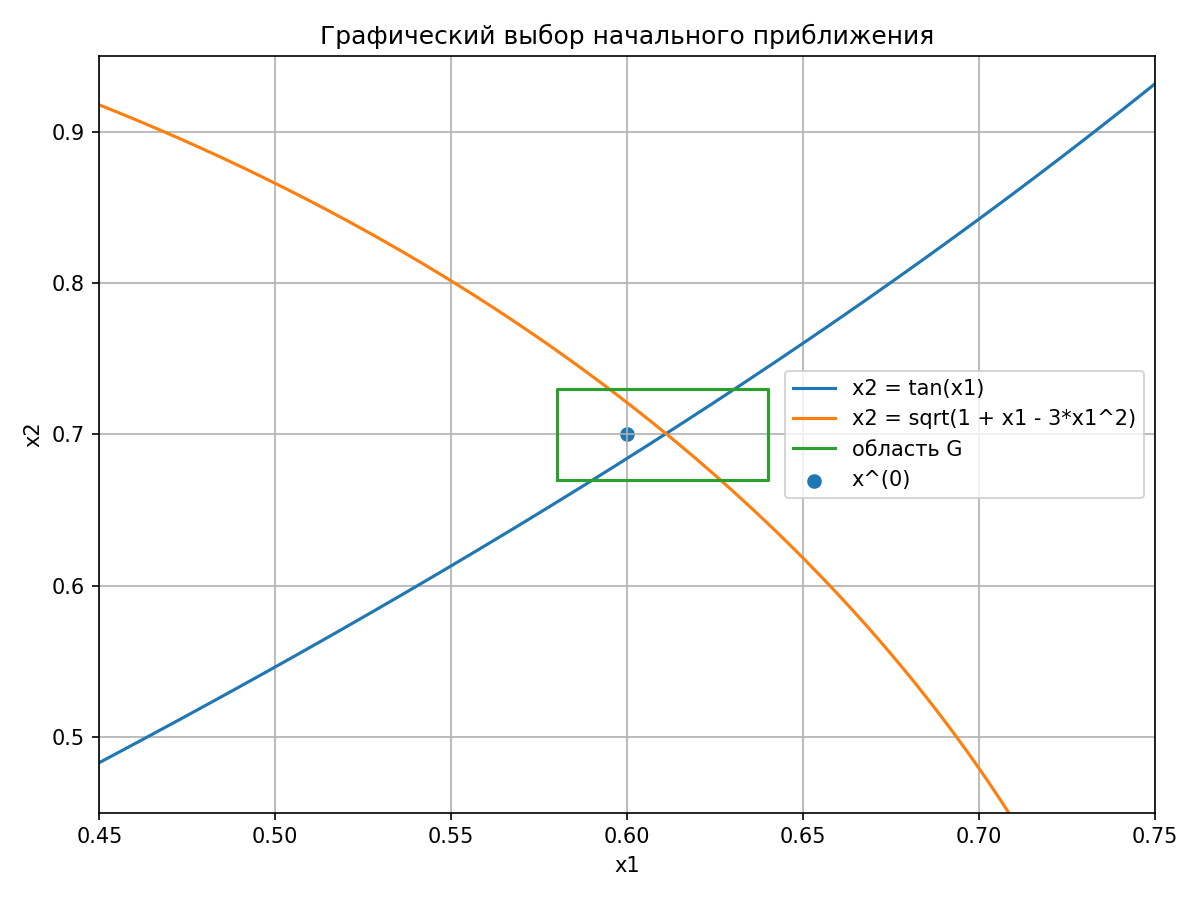
\includegraphics[width=0.68\textwidth]{lab2_2_graph.png}
    \caption{Графический выбор начального приближения}
\end{figure}

\subsubsection{Текст программы}
\programwithoutput{lab2/2_2.py}{report_outputs/2_2.txt}

\subsubsection{Анализ сходимости}
Для метода простой итерации программа вычислила
$q=0.0903973619<1$, следовательно, процесс сходится в области $G$.
Метод Ньютона дал решение
\[
x_1=0.6110978165,\qquad x_2=0.7005542039,
\]
а метод простой итерации ---
\[
x_1=0.6110978696,\qquad x_2=0.7005542250.
\]
\begin{figure}[H]
    \centering
    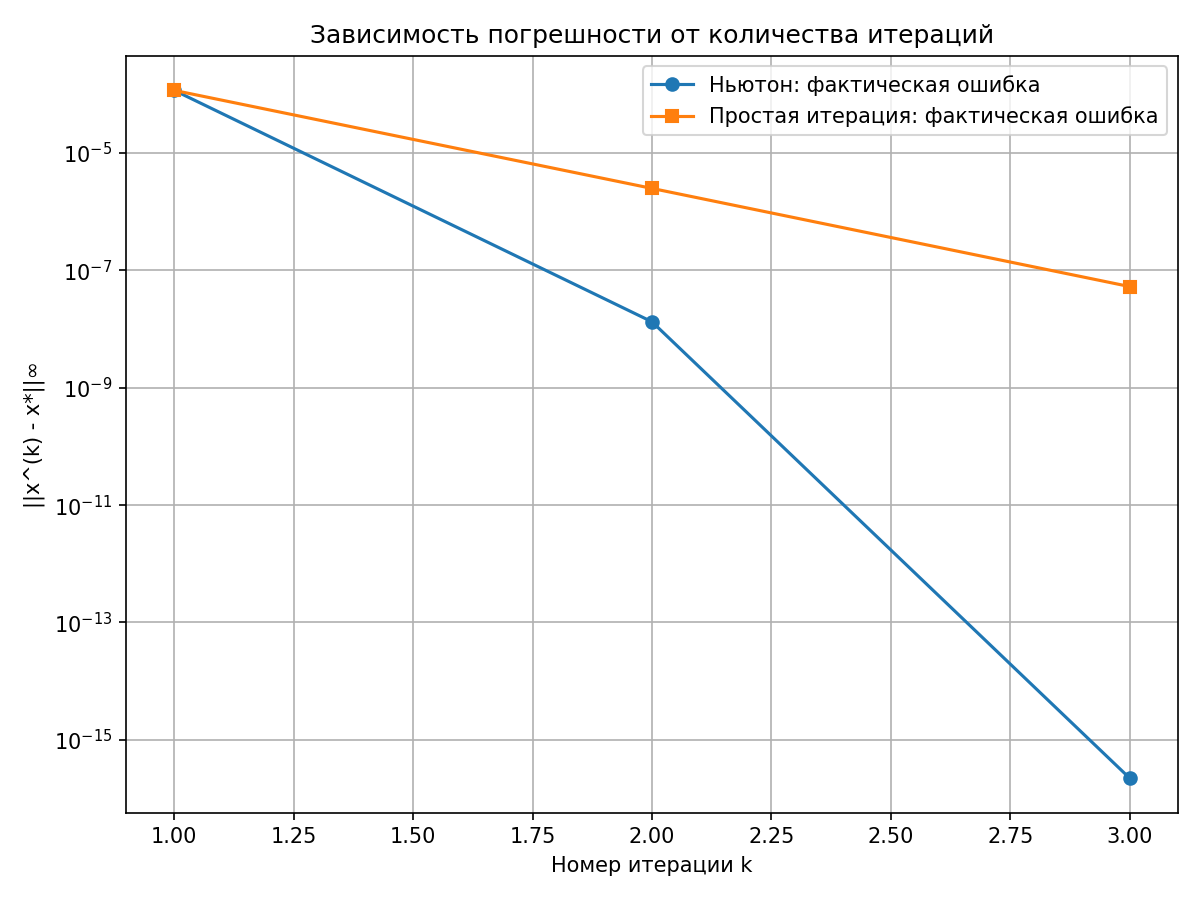
\includegraphics[width=0.68\textwidth]{lab2_2_errors.png}
    \caption{Зависимость погрешности от количества итераций}
\end{figure}

\subsection{Выводы}
Для скалярного уравнения и системы нелинейных уравнений реализованы два
итерационных подхода. Условия сходимости проверены численно на выбранных
отрезке и области. Полученные решения методов Ньютона и простой итерации
согласуются в пределах требуемой точности.

\section{Интерполяция и аппроксимация}

\subsection{Задание 3.1}

\subsubsection{Формулировка задания}
Построить интерполяционные многочлены Лагранжа и Ньютона, вычислить их
значения в заданной точке и оценить абсолютную погрешность.

\subsubsection{Вариант № 24}
Задана функция
\[
f(x)=\frac{1}{x^2},\qquad X^*=0.8,
\]
и два набора узлов:
\[
\text{а)}\ (0.1,\ 0.5,\ 0.9,\ 1.3),\qquad
\text{б)}\ (0.1,\ 0.5,\ 1.1,\ 1.3).
\]

\subsubsection{Основные формулы}
Интерполяционный многочлен Лагранжа:
\[
L_n(x)=\sum_{i=0}^{n}f(x_i)
\prod_{\substack{j=0\\j\ne i}}^{n}\frac{x-x_j}{x_i-x_j}.
\]
Интерполяционный многочлен Ньютона:
\[
P_n(x)=f[x_0]+\sum_{i=1}^{n}f[x_0,\ldots,x_i]
\prod_{j=0}^{i-1}(x-x_j).
\]

\subsubsection{Текст программы}
\programwithoutput{lab3/3_1.py}{report_outputs/3_1.txt}

\subsubsection{Анализ результатов}
Для каждого набора узлов формы Лагранжа и Ньютона совпали с точностью
округления. В случае а) абсолютная ошибка в точке $X^*$ составила
$3.3946279860$, а в случае б) --- $8.2210163089$. Поэтому для данной точки
первый набор узлов даёт более точную интерполяцию.

\subsection{Задание 3.2}

\subsubsection{Формулировка задания}
Построить естественный кубический сплайн по заданной таблице значений и
вычислить значение сплайна в указанной точке.

\subsubsection{Вариант № 24}
\[
\begin{array}{c|ccccc}
x_i&0.1&0.5&0.9&1.3&1.7\\ \hline
f_i&100.00000&4.00000&1.23460&0.59172&0.34602
\end{array},
\qquad X^*=0.8.
\]

\subsubsection{Основные формулы}
На отрезке $[x_{i-1},x_i]$ сплайн имеет вид
\[
S_i(x)=a_i+b_i(x-x_{i-1})+c_i(x-x_{i-1})^2+d_i(x-x_{i-1})^3.
\]
Коэффициенты находятся из условий интерполяции и гладкости, а для
естественного сплайна дополнительно задаются условия
\[
S''(x_0)=0,\qquad S''(x_n)=0.
\]

\subsubsection{Текст программы}
\programwithoutput{lab3/3_2.py}{report_outputs/3_2.txt}

\subsubsection{Анализ результатов}
Точка $X^*=0.8$ находится на отрезке $[0.5,0.9]$. Для найденных
коэффициентов программа получила
\[
S(0.8)=-1.8978470703.
\]

\subsection{Задание 3.3}

\subsubsection{Формулировка задания}
Методом наименьших квадратов построить приближающие многочлены первой и
второй степени для таблично заданной функции. Сравнить суммы квадратов
ошибок и построить график.

\subsubsection{Вариант № 24}
\[
\begin{array}{c|rrrrrr}
x_i&0.1&0.5&0.9&1.3&1.7&2.1\\ \hline
y_i&100.00000&4.00000&1.23460&0.59172&0.34602&0.22676
\end{array}.
\]

\subsubsection{Основные формулы}
Для $F_m(x)=a_0+a_1x+\ldots+a_mx^m$ коэффициенты находятся из условия
\[
\Phi(a_0,\ldots,a_m)=\sum_{i=0}^{n}(F_m(x_i)-y_i)^2\longrightarrow\min.
\]
Нормальная система имеет вид
\[
\sum_{j=0}^{m}a_j\sum_{i=0}^{n}x_i^{j+k}
=\sum_{i=0}^{n}y_ix_i^k,\qquad k=0,\ldots,m.
\]

\subsubsection{Текст программы}
\programwithoutput{lab3/3_3.py}{report_outputs/3_3.txt}

\subsubsection{График аппроксимации}
\begin{figure}[H]
    \centering
    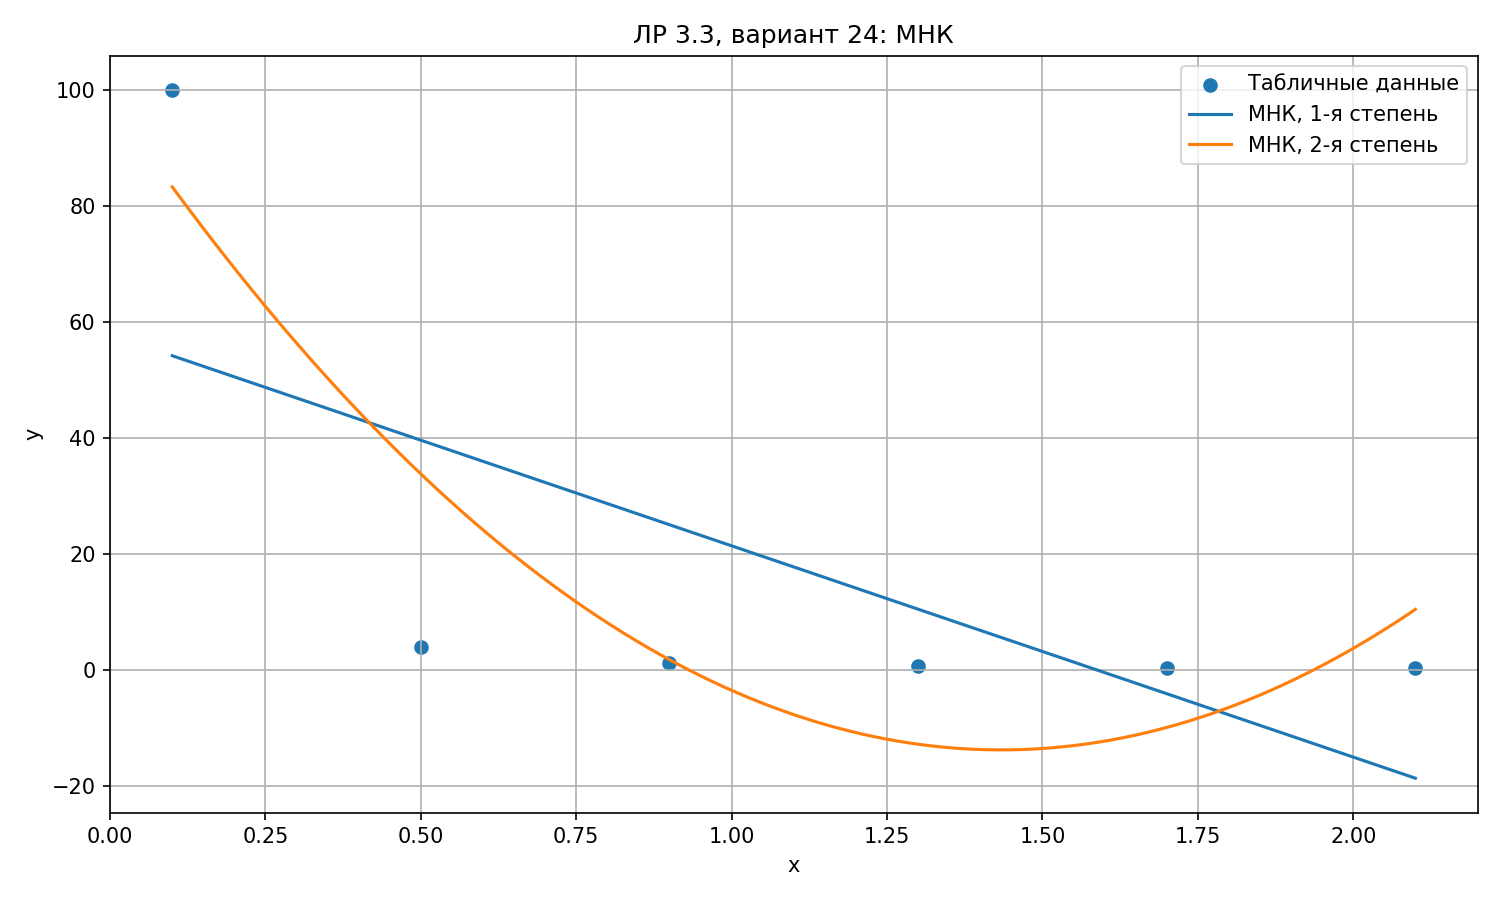
\includegraphics[width=0.76\textwidth]{3_3.png}
    \caption{Аппроксимация табличных данных методом наименьших квадратов}
\end{figure}

\subsubsection{Анализ результатов}
Получены многочлены
\[
F_1(x)=57.84162062-36.46221571x,\qquad \Phi_1=4408.66988343,
\]
\[
F_2(x)=98.44972981-156.64765098x+54.62974330x^2,\qquad
\Phi_2=1556.37086193.
\]
Так как $\Phi_2<\Phi_1$, лучшим из исследованных приближений является
многочлен второй степени.

\subsection{Задание 3.4}

\subsubsection{Формулировка задания}
По табличным значениям функции вычислить первую и вторую производные в
указанной точке с использованием формул численного дифференцирования.

\subsubsection{Вариант № 24}
\[
\begin{array}{c|ccccc}
x_i&1.0&1.2&1.4&1.6&1.8\\ \hline
y_i&2.0000&2.1344&2.4702&2.9506&3.5486
\end{array},
\qquad X^*=1.4.
\]

\subsubsection{Основные формулы}
Для равномерной сетки с шагом $h$ центральные формулы имеют вид
\[
y'(x_i)\approx\frac{y_{i+1}-y_{i-1}}{2h},\qquad
y''(x_i)\approx\frac{y_{i+1}-2y_i+y_{i-1}}{h^2}.
\]

\subsubsection{Текст программы}
\programwithoutput{lab3/3_4.py}{report_outputs/3_4.txt}

\subsubsection{Анализ результатов}
При $h=0.2$ вычислены значения
\[
y'(1.4)\approx2.040500,\qquad y''(1.4)\approx3.615000.
\]

\subsection{Задание 3.5}

\subsubsection{Формулировка задания}
Вычислить определённый интеграл методами прямоугольников, трапеций и
Симпсона на двух сетках. Уточнить результат методом Рунге--Ромберга.

\subsubsection{Вариант № 24}
\[
I=\int_{-2}^{2}\sqrt{16-x^2}\,dx,\qquad h_1=1,\qquad h_2=0.5.
\]

\subsubsection{Основные формулы}
Составные квадратурные формулы на равномерной сетке:
\[
I_{\text{пр}}=h\sum_{i=0}^{N-1}
f\left(\frac{x_i+x_{i+1}}{2}\right),
\]
\[
I_{\text{тр}}=h\left(\frac{f_0+f_N}{2}+\sum_{i=1}^{N-1}f_i\right),
\]
\[
I_{\text{С}}=\frac{h}{3}
\left(f_0+f_N+4\sum_{\text{нечётн. }i}f_i+
2\sum_{\substack{\text{чётн. }i\\i\ne0,N}}f_i\right).
\]
Уточнение Рунге--Ромберга:
\[
I_{\text{RR}}=I_{h_2}+\frac{I_{h_2}-I_{h_1}}{2^p-1}.
\]

\subsubsection{Текст программы}
\programwithoutput{lab3/3_5.py}{report_outputs/3_5.txt}

\subsubsection{Анализ результатов}
Точное значение равно $15.30578364$. После уточнения Рунге--Ромберга
наименьшую абсолютную ошибку показала формула Симпсона:
\[
|I-I_{\text{RR}}|=0.00001696.
\]

\subsection{Выводы}
Реализованы методы интерполяции, сплайн-аппроксимации, наименьших квадратов,
численного дифференцирования и интегрирования. Эквивалентные формы
интерполяционного многочлена дали одинаковые значения. В задаче МНК
квадратичный многочлен лучше линейного по сумме квадратов невязок. При
вычислении интеграла наиболее точным оказался метод Симпсона с уточнением.

\section{Решение дифференциальных уравнений}

\subsection{Задание 4.1}

\subsubsection{Формулировка задания}
Решить задачу Коши для обыкновенного дифференциального уравнения второго
порядка методами Эйлера, Рунге--Кутты и Адамса. Оценить погрешность методом
Рунге--Ромберга и сравнением с точным решением.

\subsubsection{Вариант № 24}
\[
x^2y''+(x+1)y'-y=0,\qquad
y(1)=2+e,\quad y'(1)=1,\quad x\in[1,2],\quad h=0.1.
\]
Точное решение:
\[
y(x)=x+1+xe^{1/x}.
\]

\subsubsection{Основные формулы}
После замены $z=y'$ задача сводится к системе
\[
y'=z,\qquad z'=\frac{y-(x+1)z}{x^2}.
\]
Явный метод Эйлера для вектора $Y=(y,z)^T$:
\[
Y_{k+1}=Y_k+hF(x_k,Y_k).
\]
Метод Рунге--Кутты четвёртого порядка:
\[
Y_{k+1}=Y_k+\frac{K_1+2K_2+2K_3+K_4}{6}.
\]
Для оценки ошибки решения порядка $p$ используется формула
\[
R_{\text{RR}}=\frac{|y_{h/2}-y_h|}{2^p-1}.
\]

\subsubsection{Текст программы}
\programwithoutput{lab4/4_1.py}{report_outputs/4_1.txt}

\subsubsection{Анализ результатов}
Максимальные ошибки по точному решению составили:
\[
\begin{array}{c|c}
\text{Метод}&\max |y_{\text{точн}}-y_h|\\ \hline
\text{Эйлера}&1.719235724\cdot10^{-2}\\
\text{Рунге--Кутты 4-го порядка}&9.868449371\cdot10^{-6}\\
\text{Адамса 4-го порядка}&1.087491096\cdot10^{-3}
\end{array}
\]
На выбранной сетке наибольшую точность обеспечил метод Рунге--Кутты
четвёртого порядка.

\subsection{Задание 4.2}

\subsubsection{Формулировка задания}
Решить краевую задачу для ОДУ второго порядка методом стрельбы и
конечно-разностным методом. Оценить погрешность методом Рунге--Ромберга и
путём сравнения с точным решением.

\subsubsection{Вариант № 24}
\[
(x^2+1)y''-2y=0,\qquad
y'(0)=2,\quad y(1)=3+\frac{\pi}{2},\quad h=0.1.
\]
Точное решение:
\[
y(x)=x^2+x+1+(x^2+1)\arctan x.
\]

\subsubsection{Основные формулы}
В методе стрельбы неизвестный параметр $\eta=y(0)$ подбирается так, чтобы
решение задачи Коши
\[
y'=z,\qquad z'=\frac{2y}{x^2+1},\qquad
y(0)=\eta,\quad z(0)=2
\]
удовлетворяло правому граничному условию. Для функции невязки
\[
\Phi(\eta)=y(1,\eta)-\left(3+\frac{\pi}{2}\right)
\]
применяется метод секущих.

В конечно-разностном методе во внутренних узлах используется аппроксимация
\[
y''(x_k)\approx\frac{y_{k+1}-2y_k+y_{k-1}}{h^2},
\]
а производная на левой границе аппроксимируется односторонней разностью.
Возникающая трёхдиагональная система решается методом прогонки.

\subsubsection{Текст программы}
\programwithoutput{lab4/4_2.py}{report_outputs/4_2.txt}

\subsubsection{Анализ результатов}
В методе стрельбы за одну итерацию секущих найден параметр
\[
\eta=y(0)=1.0000045178.
\]
Его максимальная ошибка на сетке составляет $4.52\cdot10^{-6}$.
Максимальная ошибка конечно-разностного решения равна $7.23\cdot10^{-2}$,
что связано с применением односторонней разности первого порядка в
граничном условии.

\subsection{Выводы}
При решении задачи Коши метод Рунге--Кутты четвёртого порядка дал
существенно меньшую погрешность, чем явный метод Эйлера и метод Адамса в
реализованной схеме. В краевой задаче метод стрельбы на той же сетке
оказался точнее конечно-разностного метода, поскольку последний теряет
порядок аппроксимации из-за обработки производного граничного условия.

\section{Итоги}
В работе реализованы и проверены численные методы четырёх основных разделов:
линейной алгебры, решения нелинейных уравнений, интерполяции и
аппроксимации, решения обыкновенных дифференциальных уравнений. Для каждого
задания представлены исходные данные варианта, расчётные формулы, полный
текст программы и фактический вывод выполнения. Результаты расчётов
подтверждают корректность реализованных алгоритмов и ожидаемые различия
между методами по скорости сходимости и точности.

\end{document}
